%% LaTeX2e class for student theses
%% thesis.tex
%% 
%% Based on SDQ KIT Template by Erik Burger
%%
%% Karlsruhe Institute of Technology
%% Institute for Automation and Applied Informatics
%% AIDA Research Group
%%
%% Nicole Ludwig
%% nicole.ludwig@kit.edu
%%
%% Version 1.3, 20.11.2018

%% Available page modes: oneside, twoside
%% Available languages: english, ngerman
%% Available modes: draft, final
\documentclass[twoside, english,figuresleft]{thesisIAI}

%% ---------------------------------
%% | Additonal Packages |
%% ---------------------------------

\input{tex/preamble}
%\usepackage[utf8]{inputenc}

\usepackage[nosuper,toc,acronyms]{glossaries}
\usepackage{url}
\usepackage{eso-pic}
\usepackage{makecell}

\newcommand\BackgroundPic{%
\put(0,0){%
\parbox[b][\paperheight]{\paperwidth}{%
\vfill
\centering
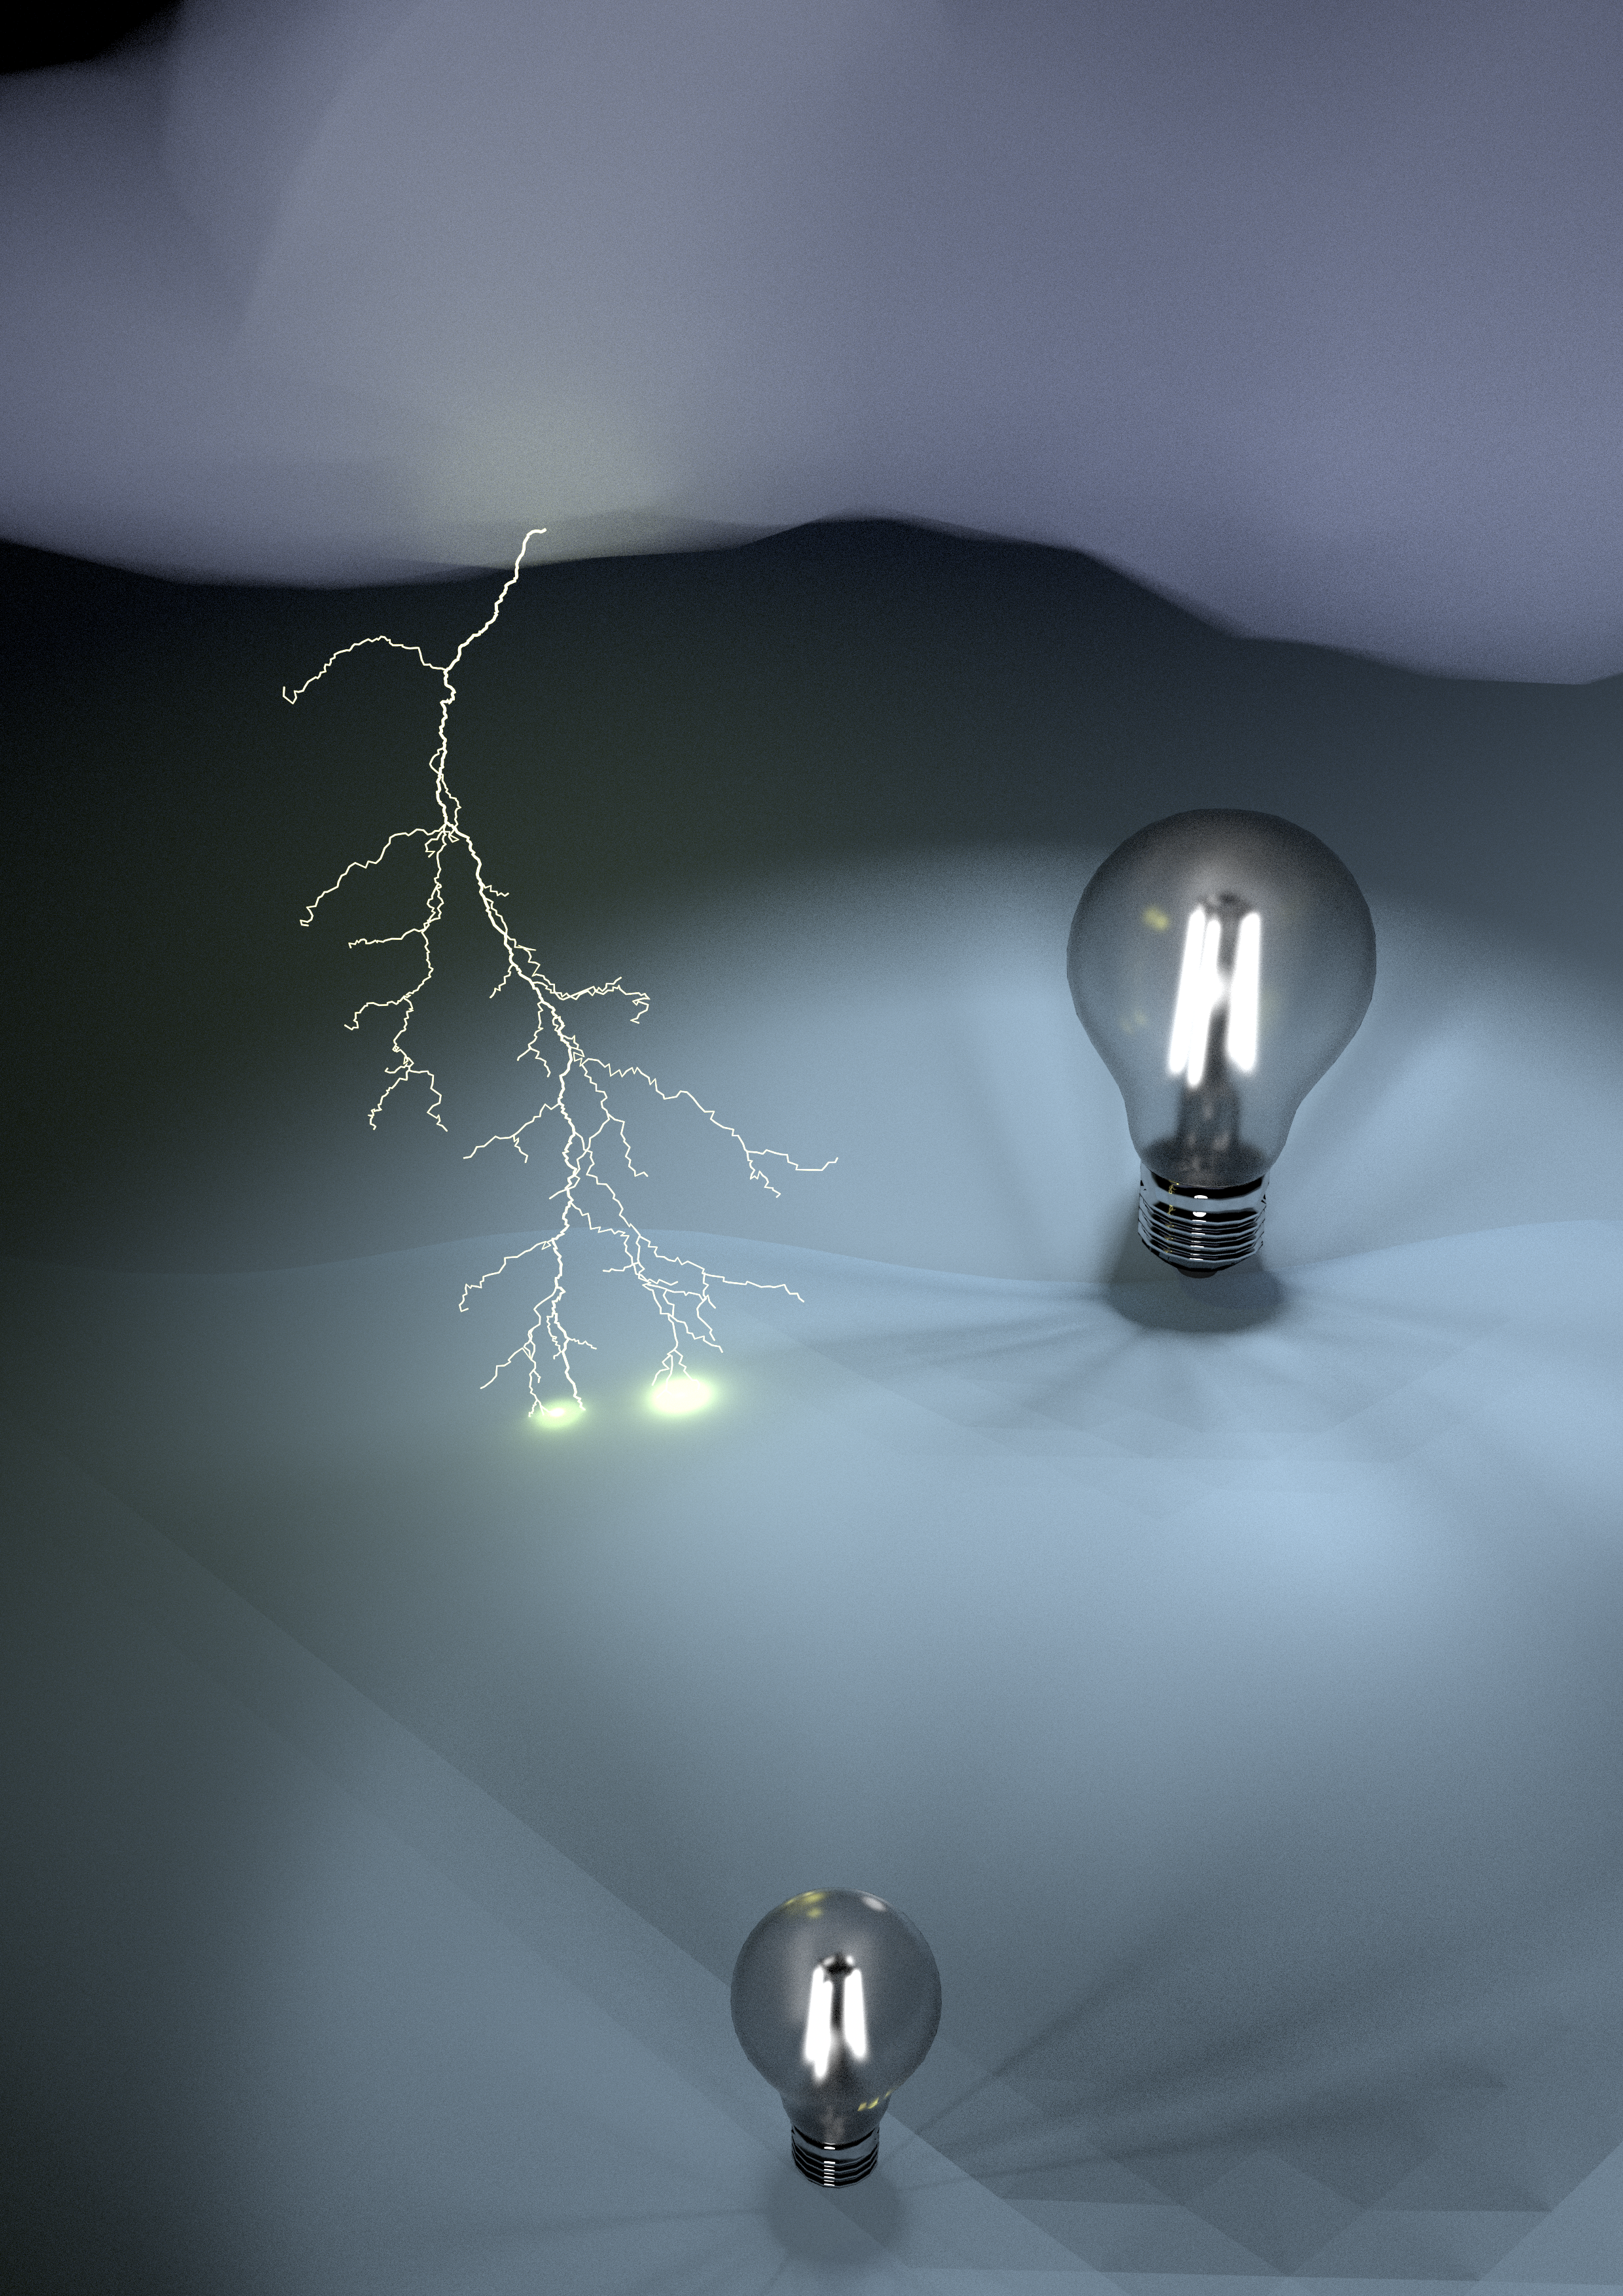
\includegraphics[width=\paperwidth,%
keepaspectratio]{logos/bulb.png}%
\vfill
}}}

\newcommand{\tcite}{\Textcite}
\newcommand{\acrs}{\acrshort}

\NewDocumentCommand{\apply}{O{,~}mm}
{% #1 = output separator, #2 = command to apply, #3 = list
  \critch_apply:Nnn { #2 } { #1 } { #3 }
}

%% ---------------------------------
%% | Information about the thesis  |
%% ---------------------------------

%% Name of the author
\author{Marcel Herm}

%% Title (and possibly subtitle) of the thesis
%\title{GIS meets energy}
\title{Evaluating the benefit of grid-based weather information in energy forecasting}

%% Type of the thesis 
\thesistype{Bachelors's Thesis}
%\thesistype{Seminar Paper}

%% Change the faculty here
%\faculty{Seminar}
%\faculty{Engineering}
\faculty{Informatics}
%\faculty{Economics}

%% The advisors are PhDs or Postdocs
\advisorone{Nicole Ludwig, M.Sc}
%% The second advisor can be omitted
\advisortwo{Marian Turowski, M.Sc}

%% Please enter the start end end time of your thesis
\editingtime{Summer Term}{2019}

\settitle

%% Please do not change anything in this tex file without talking to your supervisor
\input{tex/formats}

%% --------------------------------
%% | Settings for word separation |
%% --------------------------------

%% Describe separation hints here.
%% For more details, see 
%% http://en.wikibooks.org/wiki/LaTeX/Text_Formatting#Hyphenation
\hyphenation{
% me-ta-mo-del
}

%% --------------------------------
%% | Bibliography                 |
%% --------------------------------

% Please make sure your bibfiles name is thesis.bib and is located in the tex subfolder
\input{tex/bibliography} 

%% --------------------------------
%% | Glossary                     |
%% --------------------------------
\makeglossaries

%\newglossaryentry{ECMWF}
%{
%  name=European Centre of Medium-Range Weather Forecasts,
%  description={a research institute and a 24/7 operational service, producing global numerical weather predictions and other data}
%}

% data sources
\newacronym{ecmwf}{ECMWF}{European Centre of Medium-Range Weather Forecasts}
\newacronym{nuts}{NUTS}{Nomenclature des Unités territoriales statistiques}
\newacronym{sdhws}{SDHWS}{Solar Domestic Hot Water Systems}

% used methods
\newacronym{pdf}{PDF}{probability density function}
\newacronym{nn}{NN}{neural network}
\newacronym{vd}{VD}{variance deficit}
\newacronym{emos}{EMOS}{Ensemble Model Output Statistics}
\newacronym{pe}{PE}{persistence ensemble}
\newacronym{lr}{LR}{linear regression}
\newacronym{svm}{SVM}{Support Vector Machine}
\newacronym{arma}{ARMA}{autoregressive moving average}
\newacronym{elm}{ELM}{Extreme Learning Machine}
\newacronym{cro}{CRO}{Coral Reefs Optimization}
\newacronym{svr}{SVR}{Support Vector Regression}
\newacronym{gga}{GGA}{Grouping Genetic Algorithm}





%% ====================================
%% ====================================
%% ||                                ||
%% || Beginning of the main document ||
%% ||                                ||
%% ====================================
%% ====================================
\begin{document}

\AddToShipoutPicture*{\BackgroundPic}

\hypersetup{pageanchor=false}

%% Set PDF metadata
\setpdf

%% Set the title
\maketitle

%% The Preamble begins here
\frontmatter

\input{sections/declaration.tex}

\setcounter{page}{1}
\pagenumbering{roman}

%% ----------------
%% |   Abstract   |
%% ----------------
 
%% For theses written in English, an abstract both in English
%% and German is mandatory.
%%
%% Seminar Papers written in English need only an English abstract.
%%
%% For theses written in German, a German abstract is sufficient.
%%
%% The text is included from the following files:
%% - sections/abstract
%% - sections/zusammenfassung

\pdfbookmark[1]{Abstract}{Abstract}

\chapter*{Abstract}

\begin{center}
  \begin{minipage}{12cm}
    \begin{sloppypar}
    	There is no doubt, that electricity demand depends more and more on local weather as the share of renewable resources in electricity generation grows. This is, why it is important to find new and more reliable ways to react on the fluctuations that become increasingly volatile. One possible way is grid-based data, such as that from the \gls{ecmwf}, which is rectified based on past measurement errors and therefore may be even more correct than actual measures from local weather stations. However, a result of this work is that including multiple single grid points does not lead to an improvement. An aggregation of points over an area, such as the mean over the whole grid for the temperature, however, is more likely to do so. This gives new insight about how to best use grid-based data in order to use weather data to improve forecasts in the energy sector.
%    	Whilst the energy transition in Germany proceeds, it gets more and more important to implement techniques, allowing to react rapidly on fluctuations in energy demand. This is important, because those fluctuations become more volatile as the dependence on weather grows. Therefore, 
%    	This is an abstract. It is fine because it is small and nice.
%		As the share of electricity from regenerative sources is growing constantly, the weather becomes an increasingly important factor in the analysis of electricity markets. Hence, this thesis uses local weather data to predict electricity spot prices. More precisely, we include wind speed and temperature from individual German weather stations into time series and statistical learning models. However, as the available weather information is vast and renewable power is not generated everywhere, we use random forests and Bayesian structural time series to perform a feature selection. Overall, we manage to improve our forecasting accuracy of the EPEX electricity prices by up to \SI{7.69}{\percent} in terms of root mean squared error and up to \SI{8.19}{\percent} in terms of mean absolute error.
    \end{sloppypar}
  \end{minipage}
\end{center}

\hypersetup{pageanchor=true}
%% ------------------------
%% |   Table of Contents  |
%% ------------------------
\tableofcontents
\listoffigures
\listoftables

%% -----------------
%% |   Main part   |
%% -----------------

\mainmatter

\chapter{Introduction}
\label{ch:Introduction}


According to \tcite{Li2009}, especially temperature and perceived temperature have a great impact on energy demand. Consequently, several authors combine forecasting energy time series using weather data. They mostly either focus on forecasting \gls{pv} electricity generation as in \tcite{Bofinger2006} and \tcite{Sperati2016} or on electricity generation from wind as in \tcite{Davo2016} and \tcite{Alessandrini2015}.\\

It is notable, that works using station-based data often try to do some sort of geographic interpolation to be able to obtain values for every possible position. Considering this thesis, there is no such problem, as the used grid-based data already provides such distributed values. Thus, when using grid-based data, the step of interpolation can be omitted, and therefore, less effort is required. Some works also regard only forecasting for specific locations or accumulated values for bigger areas. With grid-based data, more general predictions can be made regarding the target location, as there is no binding to a certain locality.\\

Another interesting point is, that the works that forecast weather related time series all used grid-based data, though some of them also used station-based data to refine their forecasts. Among the papers that aimed for forecasting power or similar often only station-based data is used which leads to the assumption that less effort has been made in these fields, as it is still more complex to acquire grid-based data. However, there remains the possibility that station-based data is more suitable, even though this means a trade-off in terms of flexibility. Of course it is also possible that this has to do with the fact, that there is no grid-based power data available as this may harm privacy issues.\\

%Your thesis should start with an introduction. The introduction is supposed to motivate your thesis.
%Discuss the relevance of your topic, why are you looking into it, why is it relevant in the field? Cite important research related to your motivation.
%Briefly state the problem as in the abstract and repeat the contribution, for example in the form of research questions. 

%Give an outline of your thesis.


%Below, you will find an example figure (\Cref{fig:example}). Please use the caption of your figures to describe everything in the figure, additionally to what you have written about the figure in the text. Everyone should be able to understand the figure just reading its caption.

%\begin{figure}[h!]%
%\centering
%\includegraphics[width=0.5\columnwidth]{plots/Figure_2_demand}%
%\caption{This is an example figure. It shows a fictional demand of energy (in grey) over time.}%
%\label{fig:example}%
%\end{figure}

%This work is supposed to refer about including grid-based data into load forecasts using different methods.\\

\chapter{Related Work}
\label{ch:RW}

In this chapter, the subject of this thesis will be compared to similar works, a few points will be outlined and considered to be either valuable in terms of relevance for this thesis. There will also be a few points about the process of research.\\

\section{Research}
\label{sec:res}

Gathering information is a key element in research. Therefor, \tcite{arXiv},\tcite{scholGoogle} and \tcite{base} have been used in order to find suitable reading.\\
As the title of a work often gives a good overview, a major criteria at searching for similar papers was if the title implies working with geographic or grid-based data and/or has an application in the field of energy networks and aims at forecasting correlating values.\\
Another criteria is the abstract and/or introduction, where a priority was to check wether the used data is grid based and if not directly mentioned in the title, if or how forecasting is done.\\
%This chapter is supposed to summarise previous work of other researchers related to your topic.
%The aim is to give an overview of existing literature while highlighting differences and similarities to this thesis.
%Please choose a coherent citation style throughout the thesis. For example
%\begin{itemize}
%	\item Direct citation of results, an approach or similar
%	%\item[] \Textcite{Fan.2015} find that their method improves the benchmark.
%	\item Indirect citation
%	\item[] Recent research highlights the importance of this method %\Parencite{Fan.2015}.
%	\item Direct citation
%	\item[] \textquote{\emph{Energy optimisation in buildings is important}} %\Parencite{Fan.2015}.
%\end{itemize}

\section{Related Work}
\label{sec:rw}

When it comes to weather based prediction of power, a lot of papers have been puplished. Some of them also used data from \gls{ecmwf}, but in the process of research, there didn't come up any that had a focus on the aspect of grid-based data.\\

As, according to \tcite{Li2009}, especially temperature and perceived temperature have a great impact on energy demand, a lot of the papers that combine forecasting energy demand or generation with using weather data are focusing either on forecasting \gls{pv} electricity generation as in \tcite{Bofinger2006} and \tcite{Sperati2016} or on electricity generation from wind as in \tcite{Davo2016} and \tcite{Alessandrini2015}.\\

In the following, a few papers will be outlined and explained regarding their type of data, used forecasting methods, the forecast horizon and their forcasted timeseries.\\

For time series forecasting, often used methods are e.g.\ \gls{arma} models as mentioned in \tcite{Hyndman2018}, but  also \gls{nn}, where it is common to reduce the number input variables in order to speed up computation, which is desirable for the huge amount of grid-based data that grows quadratically with size. Last there are also some papers that use regression models other than \gls{arma} such as simple \gls{lr},\gls{mlr} or \gls{svm}.\\\
E.g.\ \tcite{Aguiar2016} uses \gls{ann} to do intra-day forecasting of solar radiation within 1-6h on Gran Canaria and, as in this thesis, data from \gls{ecmwf} is used.\\
\tcite{Alessandrini2015} proposes a novelty by applying an \gls{anen} method to retain a probabilistic wind power forecast. Here the data from \gls{ecmwf} is indirectly used by feeding it into the \gls{rams} to get forecast data for the prediction. The temporal forecast horizon in this case is also rather short with 0-132h of probabilistic forecasting.\\
\tcite{Bofinger2006} also used data from \gls{ecmwf}, but also data from local weather stations to forecast solar power output within a 24-120h range. The data is then refined using \gls{mos} and \gls{idw}, spatially interpolated and then simulated for germany.\\
Another paper that used data from \gls{ecmwf} is \tcite{Davo2016}. Here also data from \gls{noaaesrl} was used which was provided for an online competition hosted by \tcite{kaggle}. Reference power data was obtained from \tcite{terna}. This is the only paper so far using \gls{pca} to reduce dimensionality, but as in \tcite{Alessandrini2015}, \gls{anen} is used, whereas here, \gls{nn} are used before. The target values here are both solar radiation and wind power produced over Sicily within a 0-72h range.\\
Similar to this thesis, \tcite{DeFelice2015} aims to forecast electricity demand using data from \gls{ecmwf}, though  for italy and with a medium-term temporal range of around 1-2 months in contrast to the short-term range targeted in this thesis. Therefor \gls{lr} and \gls{svm} are used. As power prediction is a rather complex problem, it is not very surprising that the non-linear \gls{svm} performs better than \gls{lr}.\\
In terms of this thesis, a very interesting paper is \tcite{Diagne2013} where different forecasting methods are reviewed, even though for solar radiation forecasting. Also different data sources are compared, specifically \gls{ecmwf},\gls{mm5} and \gls{wrf}. The paper focuses on \gls{ar} methods including \gls{arma},\gls{arima} and \gls{cards} and \gls{nn} with \gls{ann} and \gls{wnn} considering short time ranges from 5 min up to 6h.\\
In contrast to that, \tcite{Ludwig2015} does not consider \gls{nn}, but therefor compares \gls{lasso} and \gls{rf} next to \gls{arma} and \gls{armax} models. The target value here is the german electricity price for the next day, thus having a 24h forecast horizon, and the used data is obtained by distributed measures from \gls{dwd} for weather data and from \gls{epex} for the price history. A desirable side effect from \gls{rf} is the output of the variable importance which is useful in order to filter variables by order of their importance.\\
An interesting work about low voltage load forecasting is \tcite{Haben2018} where \gls{kde},\gls{sslr},\gls{arwd},\gls{arwdy} and \gls{hwt} are comepared for a forecast horizon of up to 4 days. The weather data used here to refine the forecasting results are station-based.\\
Further methods are presented in \tcite{Salcedo-Sanz2018} with combinations of \gls{cro},\gls{elm},\gls{gga},\gls{mars},\gls{svr} for short-term solar radiation forecast of 24h in Australia. The used data comes mostly from \gls{ecmwf}, but also from \gls{silo} and thus uses gridded as well as non-gridded data.\\
Another application of \gls{ecmwf} data is proposed in \tcite{Sperati2016} for short-term solar power forecasting within a 0-72h time range using a \gls{pdf} combined with \gls{nn},\gls{vd},\gls{emos} and \gls{pe}.\\

%Other works regarding \gls{arima} models such as \tcite{Kaminska-Chuchmala2014} are also considered valuable information sources, though using these methods e.g.\ in this case to forecast internet traffic load which is quite similar to power demand, as the internet as well as the german power network both are supposed to work bidirectional with future regard.\\
Of course there where other papers considered such as \tcite{Kaminska-Chuchmala2014} in particular due to its subject of forecasting internet traffic load and the high correlation between internet traffic load and electricity load \Parencite{Morley2018}. The use of \gls{ok} is also interesting, but not used in this thesis, which is why this subject has not been considered for further research. Another great example would be \tcite{Fairley2017} where spatio-temporal variation in wave power and its implications for electricity supply are being discussed which combines localization issues and the electricity network, but unfortunately in this case the aim is not to forecast but only to examine the problem.\\

\Cref{tab:relwork} provides an overview about some of the mentioned related works including further information in terms of spatial distribution of the used data that does not correspond to the target value, used methods, origin of the data, temporal scope and the target value.\\
%It is to mention that regarding the temporal scope, short term means up to a few days, middle term refers to up to a few months and long term is about seasonal forecasting which possibly includes multiple years.\\

% TODO add location column?!
\begin{sidewaystable}[!ht]%
\rowcolors{2}{white}{gray!25}
\centering
\footnotesize
\begin{tabularx}{\linewidth}{llLlL}
\tablehead paper & \tablehead type of data & \tablehead methods & \tablehead forecast horizon & \tablehead forecasted timeseries \\\hline
\tcite{Aguiar2016} & grid-based & \gls{nn} & 1-6h & solar radiation\\
\tcite{Alessandrini2015} & station-based & \gls{anen} & 0-132h & wind power\\
\tcite{Bofinger2006} & mixed & \gls{mos},\gls{idw} & 24-120h & solar power\\
\tcite{Davo2016} & grid-based & \gls{pca},\gls{anen},\gls{rams} & 0-72h & wind power,solar radiation\\
\tcite{DeFelice2015} & grid-based & \gls{lr},\gls{svm} & 1-2 months & electricity demand\\
\tcite{Diagne2013} & grid-based & \gls{arma},\gls{arima},\gls{cards},\gls{ann},\gls{wnn} & 5 min-6h & solar radiation\\
\tcite{Haben2018} & station-based & \gls{kde},\gls{sslr},\gls{arwd},\gls{arwdy},\gls{hwt} & up to 4 days & low voltage electricity load\\
\tcite{Ludwig2015} & station-based & \gls{arma},\gls{armax},\gls{lasso},\gls{rf} & 24h & energy prices\\
\tcite{Salcedo-Sanz2018} & mixed & \gls{elm},\gls{cro},\gls{mars},\gls{mlr},\gls{svr},\gls{gga} & 24h & solar radiation\\
\tcite{Sperati2016} & grid-based & \gls{pdf},\gls{nn},\gls{vd},\gls{emos},\gls{pe} & 0-72h & solar power\\
%\tcite{Aertsen2012} & mixed & \gls{ok},\gls{ck},\gls{rk} & long term & TODO\\ %  maybe not relevant du to only considerinng station-based measures and thus using interpolation methods (kriging)
%\tcite{Kaminska-Chuchmala2014} & distributed &  & & & \\
%\tcite{Fairley2017} & grid?! & methods?! & \gls{ecmwf} & none?! & TODO\\ % no forecast
%\tcite{Voivontas1998} & grid?! & & \gls{sdhws} & none?! & TODO\\
\end{tabularx}
\caption{List of related works and used methods respectively as well as some further details.}
\label{tab:relwork}
\end{sidewaystable}

One key difference of the presented works to this thesis is that here, reanalyzed data from \gls{ecmwf} is used for prediction which means, that the forecasts might behave differently from forecasts in other works. This also means that results from this thesis possibly won't exactly match results using the same procedure with real-time data.\\


\chapter{Methodology}
\label{ch:methods}

%This chapter should introduce to the theoretical background of your thesis. Any method you use to obtain the results later should be introduced and explained. 
In this chapter, the used forecasting methods are explained further and why they were used, but also other methodological aspects of this thesis will be outlined.\\

%Using weather data from ECMWF Copernicus Climate Change Service (C3S).\\
%Using load data from \url{https://data.open-power-system-data.org/}.\\
%First downloaded whole Datasets from 2006-2019, but as the load for germany is properly available since 2015, now reduced dataset to 2015-2019.\\
%Also checked for non-existing values, only 2 last timestamps values for the load are missing.\\

\section{Data acquisition}
\label{sec:dataq}

In order to acquire the needed weather data, \gls{ecmwf}'s Python-API is used for automated data acquisition. The API has been extended by some functionality recently and allows to download the data with different extensions. The chosen extension is .nc, because Python's xarray library allows performant access to these files.\\

\section{Forecasting methods}
\label{sec:forecastmet}

For time series forecasting, often used methods are \eg \gls{arma} models as mentioned in \tcite{Hyndman2018}, but  also \gls{nn}, where it is common to reduce the number of input variables in order to speed up computation, which is desirable for the huge amount of grid-based data that grows quadratically with size. There are also some papers that use regression models other than \gls{arma} such as \gls{lr}, \gls{mlr} or \gls{svm}.\\
\tcite{Aguiar2016} applies \gls{nn} to do intra-day solar radiation forecasting with a forecasting horizon of 1-6 hours on Gran Canaria and, as in this thesis, grid-based data from \gls{ecmwf} is used.\\

%\subsection{Linear Regression}
\subsection{ARMA}

One of the most frequently used methods for forecasting in time series forecasting is \gls{arma}, which is a combination of \gls{ar} and \gls{ma} terms. \gls{arima} is quite similar to this, but involves an additional differentiation term to consider the trend of past data. The formal description of an \gls{arma} is given as follows:\\

\begin{equation}
y_t = c+\epsilon_t+\sum_{i=1}^{p}a_iy_{t-i}+\sum_{j=1}^{q}b_j\epsilon_{t-j}
\label{eq:arma}
\end{equation}

With $c$ as a constant, $\epsilon_t$ as noise terms with respect to time $t$, $p$ as size of the \gls{ar} part, $q$ as size of the \gls{ma} part, $a$ and $b$ for the \gls{ar} and \gls{ma} coefficients respectively and $y_t$ as the predicted value.\\

\subsection{ARMAX}

Another similar method is \gls{armax}, which includes an additional term for exogenous variables. This term can be used to include relations to external factors that do not depend on the endogenous data. The formal description is given by:\\

\begin{equation}
y_t = c+\epsilon_t+\sum_{i=1}^{p}a_iy_{t-i}+\sum_{j=1}^{q}b_j\epsilon_{t-j}+\sum_{k=1}^{n}c_kx_k
\label{eq:armax}
\end{equation}

Which almost equals to \Cref{eq:arma} for the \gls{arma}. There is an additional term for $n$ included exogenous variables $x$ with $c$ as the respective coefficients.

%\subsubsection{only calendar variables as exogenous inputs}
%
%\subsubsection{additional weather variables as exogenous inputs}

\section{Feature Selection}
\label{sec:featsel}

\subsection{Principal Component Analysis}

\section{Forecast Evaluation}
\label{sec:fceval}

\subsection{Root Mean Squared Error}

\begin{equation}
RMSE = \sqrt{\frac{1}{n} \sum_{i=1}^{n} (a_i-p_i)^2}
\label{eq:rmse}
\end{equation}

With $n$ for the size, a for the actual values and p for predicted values.\\

\subsection{Mean Absolute Percentage Error}

\begin{equation}
MAPE = \frac{1}{n}\times 100 \sum_{i=1}^{n} \left|\frac{a_i-p_i}{a_i}\right|
\label{eq:mape}
\end{equation}

With $n$ for the size, a for the actual values and p for predicted values.\\

%Maybe use Random Forests for variable selection as in Nicoles paper? \Parencite{Ludwig2015}\\

%This is an example for a simple equation without equation numbering.
%$$
%\sum\limits_{i=1}^{n}{x_i}
%$$

%You can also use equation numbering if you need to refer to an equation later \eg \Cref{eq:ex1}.


%\begin{equation}
%a^2 + b^2 = c^2
%\label{eq:ex1}
%\end{equation}
%
%Additionally, simple equations can be put inline with the text, for example, $x \in X$. Remember to set all variables in math font \ie all $x$, $i$ and so on.
%
%\section{Method 2}
%
%\dots


\chapter{Evaluation}
\label{ch:Evaluation}

\section{Data}
\label{sec:data}

Of course choosing data sources as well as sorting and cleaning the data also requires a certain amount of time and effort. Thus it will be explained hereinafter how this has been done for the data used in this thesis.

\subsection{ECMWF}

The data used in this thesis originates from \acrshort{ecmwf}, which is a research institute that produces global numerical weather predictions and other data.\\
It is time series based and for each timestamp there is a 2-dimensional array referred to by longitude and latitude respectively.\\

It must be mentioned that, as the data used has been reanalized, so the expected error is likely to be smaller than if working with real-time data.\\

As data parameters there are also longitude and latitude, where the longitude is chosen to be from 5.5 to 15.5 and the latitude from 47 to 55.5. As the resolution of the used grid is at 0.25°, this results in a total of 1435 grid points per timestamp. As the range of the data from \acrshort{ecmwf} extends from 2015/1/1 to 2019/3/31(TODO update), there is a total of 1551 days with each 12 timestamps due to the 2 hours frequency and thus 18612 timestamps. Considering that there is a value for each point in the grid and every timestamp, there are 26708220 values for each variable.\\

In order to reduce complexity, a shapefile of the \acrshort{nuts} dataset was used. The shapefile contains all countries in the EU. The shape of germany was filtered from this data and each point in the \acrshort{ecmwf} dataset is checked wether it is within germany or not. The result can be seen in \Cref{fig:isin}.\\


\begin{figure}[h!]%
\centering
\includegraphics[width=0.8\textwidth]{plots/isin}%
\caption{2D boolean numpy.ndarray used to filter grid squares that are within germany. It was created by using a shapefile of germany (TODO insert source \url{https://ec.europa.eu/eurostat/cache/GISCO/distribution/v2/nuts/nuts-2016-files.html}) and checking for each point of the grid if it is within the shapefile. (TODO shorter explanation, put explanation in text)}%
\label{fig:isin}%
\end{figure}

\begin{figure}[h!]%
\centering
\includegraphics[width=\textwidth]{plots/0_2017010702_20190617161317}%
\caption{Map showing day with lowest temperature in germany.}%
\label{fig:0_2017010702_20190617161317}%
\end{figure}

\begin{figure}[h!]%
\centering
\includegraphics[width=\textwidth]{plots/t2m/bundles/maxvar4_maps}%
\caption{Map showing 4 times with highest temperature variance in germany, where top left is highest, top right second highest, bottom left third highest and bottom right fourth highest variance (TODO put this in text).}%
\label{fig:maxvar4_maps}%
\end{figure}



\begin{table}[h!]%
\rowcolors{2}{gray!25}{white}
\centering
\footnotesize
\begin{tabular}{llrr}
\tablehead variable name & \tablehead units & \tablehead min & \tablehead max \\\hline
10 metre U wind component & $m~s^{-1}$ & -18.56 & 21.92 \\
10 metre V wind component & $m~s^{-1}$ & -21.51 & 20.00 \\
2 metre temperature & $K$ & 240.97 & 313.26 \\
Leaf area index, high vegetation & $m^{2}~m^{-2}$ & 0.00 & 4.90 \\
Leaf area index, low vegetation & $m^{2}~m^{-2}$ & 0.00 & 3.84 \\
Low cloud cover & $(0~-~1)$ & 0.00 & 1.00 \\
Soil temperature level 1 & $K$ & 257.91 & 313.64 \\
Surface latent heat flux & $J~m^{-2}$ & -2203977.00 & 359411.00 \\
Surface net thermal radiation & $J~m^{-2}$ & -663417.00 & 142945.02 \\
Surface sensible heat flux & $J~m^{-2}$ & -1703159.00 & 801354.00 \\
Total cloud cover & $(0~-~1)$ & 0.00 & 1.00 \\
Total column rain water & $kg~m^{-2}$ & 0.00 & 2.73 \\
Total sky direct solar radiation at surface & $J~m^{-2}$ & -0.12 & 3088320.00 \\
\end{tabular}
\caption[List of exogenous weather variables used to forecast the load including min, max values from \gls{ecmwf}.]{List of exogenous weather variables used to forecast the load including min, max values from \tcite{ecmwf}.}
\label{tab:wvars}
\end{table}


\subsection{Load data}

\begin{figure}[h!]%
\centering
\includegraphics[width=\textheight,angle=-90,origin=c]{plots/t2m_mean_2015010112_2018123112_24F}%
\caption{Load curve with mean of 2 meter height measured temperature in germany as color from 2015/1/1 to 2018/12/31 with one single point per day at 12am utc time respectively.}%
\label{fig:t2m_mean_2015010112_2018123112_24F}%
\end{figure}

The load data has been retained from \tcite{opsdata}.\\
\Cref{fig:t2m_mean_2015010112_2018123112_24F} shows the distribution of loads over time with one point per day at 12am utc time. The color shows the mean temperature measured at 2 meters height.\\

%Describe the data set you are using. Use appropriate visualization (\eg graphs, statistical summaries \etc) to help the reader get to know your data set.

%\Cref{tab:wvars} is an example table. Remember to use full sentences in your caption and explain everything one can see in the table there as well. You can of course also use a simpler format for your table.


\subsection{Population}

\begin{figure}[h!]%
\centering
\includegraphics[width=\textwidth]{plots/demo/demo2018_logscale}%
\caption{Population of germany for each region respectively using a log scale for better distinction.}%
\label{fig:demo2018_logscale}%
\end{figure}


%\begin{table}[h!]%
%\caption{Example table with rotated table heads to save space and two different row colours to ease the readability.}
%\rowcolors{2}{gray!25}{white}
%\centering
%\footnotesize
%\begin{tabular}{lll}
%\toprule \noalign{\smallskip}
%\rottblhead{\tablehead Header 1} & \rottblhead{\tablehead Header 2} & \rottblhead{\tablehead Header 3} \\ \midrule
%entry 1 & entry 2 & entry 3 \\ 
%entry 1 & entry 2 & entry 3 \\ 
%entry 1 & entry 2 & entry 3 \\ 	\bottomrule
%\end{tabular}
%\label{tab:example}
%\end{table}


\section{Programming part}
\label{sec:prog}

\subsection{Programming Language}

For the programming part, Python3.6+ has been chosen, as there is a variety of libraries to process all used file formats and because it tends to be a time saving language, also for visualization.\\

\subsection{Documentation}

In regard to coding styles, especially when it comes to docstrings, the numpy conventions were used. The three major points for this were first, that it is a popular and often used style, then it is also a visually oriented style which means, that it is easy to read and last it is supported by several (TODO check which, sphinx?!) autodoc tools that create a HTML based documentation from existing source code with docstrings.\\


\section{Results}
\label{sec:results}

Describe the results you have obtained using your methods described above. Again use proper visualization methods.

\subsection{Experiment 1}

\dots

\subsection{Experiment 2}

\dots
\chapter{Discussion}
\label{ch:discussion}

Considering the main research question of this thesis, whether grid-based weather information does have a benefit on energy forecasting, it is now possible to approach an answer. As already pointed out in \Cref{sec:results}, using the actual grid points themselves does not result in any improvement, but rather causes the results to deteriorate. This seems to suggest that there is no benefit at all in using grid-based data for energy forecasting. However, grid-based data can be very useful when it is being conglomerated or compressed in a representative form, such as the mean over the longitude and latitude. This can also be observed in \Cref{sec:results}, where the averaged 2 metre temperature actually improves the forecast accuracy. The special upside in using grid-based data, such as the data from \gls{ecmwf}, is, that it can be conglomerated over any desired locality as it is available for most locations. This allows it to be used for forecasts at arbitrary locations. Even though, from the missing results of most of the given weather variables, it can not be said which of them are most suitable to be used as inputs for energy forecasting. Also, there was too much effort invested in analysing the used data which was not necessary. The spent time would have better been used to examine further model sizes or checking which weather variables improve the forecast accuracy. Another critical point is the missing of alternative methods. In this thesis, only \gls{arma} and \gls{armax} models have been used, but it is still unclear if there are better methods for energy related time series forecasting.\\
%outlook: try other methods to compress the data as representative as possible, mean over highest populated regions, or regions filtered by economic activity also compressed or so
%Looking at the results from \Cref{sec:results}, 

%This chapter is supposed to discuss your results. Point out what your results mean.
%What are the limitations of your approach, managerial implications or future impact?
%
%Explain the broader picture but be critical with your methods.
\chapter{Conclusion}
\label{ch:Conclusion}

It needs to be clarified, that in contrast to most of the presented works, this thesis uses reanalysed data from \gls{ecmwf} as weather predictions which means, that the forecasts might behave differently from forecasts in other works as what here is assumed to be a weather forecast is more accurate than usually. This also means that results from this thesis may not exactly match results using the same procedure with real-time data.\\

%Repeat the problem and its relevance, as well as the contribution (plus quantitative results). 
%Look back at what you have written in the introduction.

%Provide an outlook for further research steps.


%% ----------------
%% |   Glossary   |
%% ----------------

\printglossary[title=Terms and abbreviations,toctitle=Terms and abbreviations,type=\acronymtype]


%% --------------------
%% |   Bibliography   |
%% --------------------

%% Add entry to the table of contents for the bibliography
\printbibliography[heading=bibintoc]

%% ----------------
%% |   Appendix   |
%% ----------------
\appendix
%% LaTeX2e class for student theses
%% appendix
%% 
%% Based on SDQ KIT Template by Erik Burger
%%
%% Karlsruhe Institute of Technology
%% Institute for Automation and Applied Informatics
%% AIDA Research Group
%%
%% Nicole Ludwig
%% nicole.ludwig@kit.edu
%%
%% Version 1.2, 2018-10-11


\iflanguage{english}
{\chapter{Appendix}}    % english style
{\chapter{Anhang}}      % german style
\label{chap:appendix}


%% -------------------
%% | Example content |
%% -------------------

\begin{figure}[h!]%
\centering
\includegraphics[width=.7\textheight,angle=-90,origin=c]{plots/t2m_mean_2015010112_2018123112_24F}%
\caption{Load curve with mean of 2 meter height measured temperature in germany as color from 2015/1/1 to 2018/12/31 with one single point per day at 12am utc time respectively.}%
\label{fig:t2m_mean_2015010112_2018123112_24F}%
\end{figure}
		
%\setcounter{figure}{0}
%		
%\begin{figure} [ht]
%  \centering
%  \caption{A figure}
%  \label{fig:anotherfigure}
%\end{figure}


\end{document}